\lab{Вынужденные колебания в электрическом контуре}

\aim{исследование вынужденных колебаний и процессов их
установления в колебательном контуре.}

\equip{В работе используются: генератор звуковых частот, осциллограф,
вольтметр, частотомер, конденсатор, катушка индуктивности, магазин
сопротивлений, универсальный мост.}

В работе исследуются колебания, возникающие в параллельном
электрическом контуре под действием внешнего гармонического генератора
тока.

При подключении к контуру внешнего источника в нём возникают колебания,
которые можно представить как суперпозицию двух синусоид \chaptereqref{2.72}: первая
с частотой собственных колебаний контура и амплитудой, экспоненциально
убывающей со временем; вторая с частотой внешнего источника и постоянной
амплитудой. Со временем собственные колебания затухают, и в контуре
устанавливаются вынужденные колебания. Амплитуда этих колебаний
максимальна при резонансе совпадении частоты внешнего сигнала с
собственной частотой контура $0$. Зависимость амплитуды установившихся
колебаний от частоты внешнего напряжения носит название
\important{«резонансная кривая».}

\labsection{А. Резонансная кривая колебательного контура.}

\begin{wrapfigure}[13]{r}{0.45\linewidth}
	\pic{0.45\textwidth}{Chapter_2/2_5_2}
	\caption{Схема установки для исследования вынужденных колебаний}
	\figmark{forced oscillations scheme}
\end{wrapfigure}
%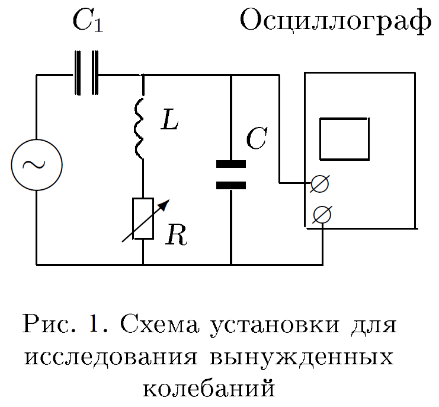
\includegraphics[width=1.99792in,height=1.85in]{./media/image1.png}
Для экспериментального исследования резонансной кривой напряжения в
параллельном колебательном контуре используется схема, изображенная на
рис.~\figref{forced oscillations scheme}. Синусоидальный сигнал с генератора подаётся на параллельный
колебательный контур через небольшую разделительную ёмкость $C_1$.
Напряжение с конденсатора контура $C$ поступает на вертикальный вход
электронного осциллографа (ЭО). Для снятия резонансной кривой
необходимо, чтобы импедансы возбуждающей и измеряющей цепей
(сопротивления переменному току) намного превосходили импеданс самого
контура вблизи резонанса $Z_{\text{рез}} \sim L/(RC) = Q/(\Omega C)$. Разделительная ёмкость
$C_1$ выбирается настолько малой, что в рабочем диапазоне частот её
импеданс $Z_{C_1} = 1/(\Omega C_1)$ много больше импеданса контура, поэтому в цепи
генератора течёт ток практически с постоянной амплитудой, а
колебательный контур выполняет роль нагрузочного сопротивления, которое,
в свою очередь, зависит от частоты. Поскольку в резонансе сопротивление
$Z_\text{рез}$ параллельного контура максимально, то и напряжение на ёмкости $C$
(неизменный ток, умноженный на максимальное сопротивление) тоже
максимально. Входное сопротивление осциллографа (измеряющей цепи)
достаточно велико: $R_{\text{ЭО}} \approx 1$~МОм, поэтому его влиянием можно пренебречь.

Таким образом, при выполнении условий

\begin{equation}
	\eqmark{2.4.1}
Z_{C_1} = \frac{1}{\Omega C_1} \gg \left| Z \right|_{rez} = \frac{Q}{\Omega C}, \qquad R_\text{ЕО} \gg \frac{Q}{\Omega C}
\end{equation}
и при условии, что действительная часть импеданса катушки много меньше
её мнимой части, резонансная кривая в нашем контуре будет выглядеть так
же, как и в последовательном: максимум амплитуды при резонансе. Ширина
резонансной кривой определяет важную характеристику контура~---~\important{добротность}.

\labsection{Б. Процессы установления и затухания колебаний в контуре.}

Добротность контура может быть определена и другими способами, например,
по скорости нарастания амплитуды вынужденных колебаний при резонансе или
по скорости затухания свободных колебаний.

\begin{wrapfigure}[13]{r}{0.45\linewidth}
	\pic{0.45\textwidth}{Chapter_2/2_5_3}
	\caption{Нарастание и затухание вынужденных колебаний}
	\figmark{forced oscillations damping}
\end{wrapfigure}
%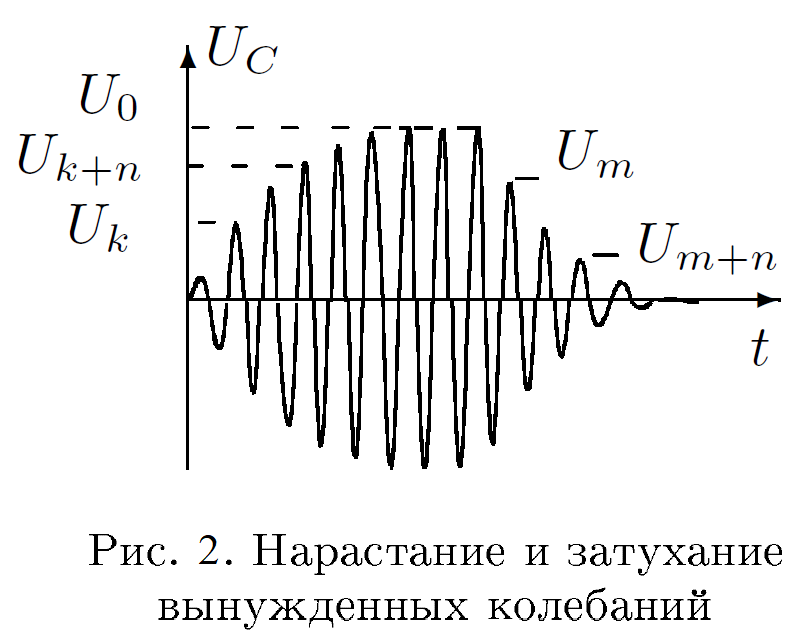
\includegraphics[width=2.72431in,height=2.17778in]{./media/image2.PNG}
Нарастание
и затухание колебаний (рис.~\figref{forced oscillations damping}) можно наблюдать на экране осциллографа,
если на контур подаются цуги~---~отрезки синусоиды, разделённые
интервалами, в течение которых сигнал отсутствует. Чем выше добротность,
тем медленнее нарастают и медленнее затухают колебания в контуре.
Количественные оценки можно сделать, если определить логарифмический
декремент затухания по скорости нарастания или затухания колебаний. В
условиях резонанса огибающая затухающих колебаний~---~это перевёрнутая
огибающая нарастающего участка, поэтому при расчёте логарифмического
декремента по затуханию нет необходимости использовать амплитуду
установившихся колебаний $U_0$, которая в контуре с высокой добротностью
может не успеть установиться за время продолжительности цуга.

\experiment Схема установки для исследования
вынужденных колебаний приведена на рис.~\figref{forced oscillations exp scheme}. Колебательный контур состоит
из конденсатора с ёмкостью $C$, катушки с индуктивностью $L$ и магазина
сопротивлений $R$.

\begin{figure}[h]
	\pic{0.45\textwidth}{Chapter_2/2_5_4}
	\caption{Схема экспериментальной установки для исследования вынужденных
колебаний}
	\figmark{forced oscillations exp scheme}
\end{figure}
%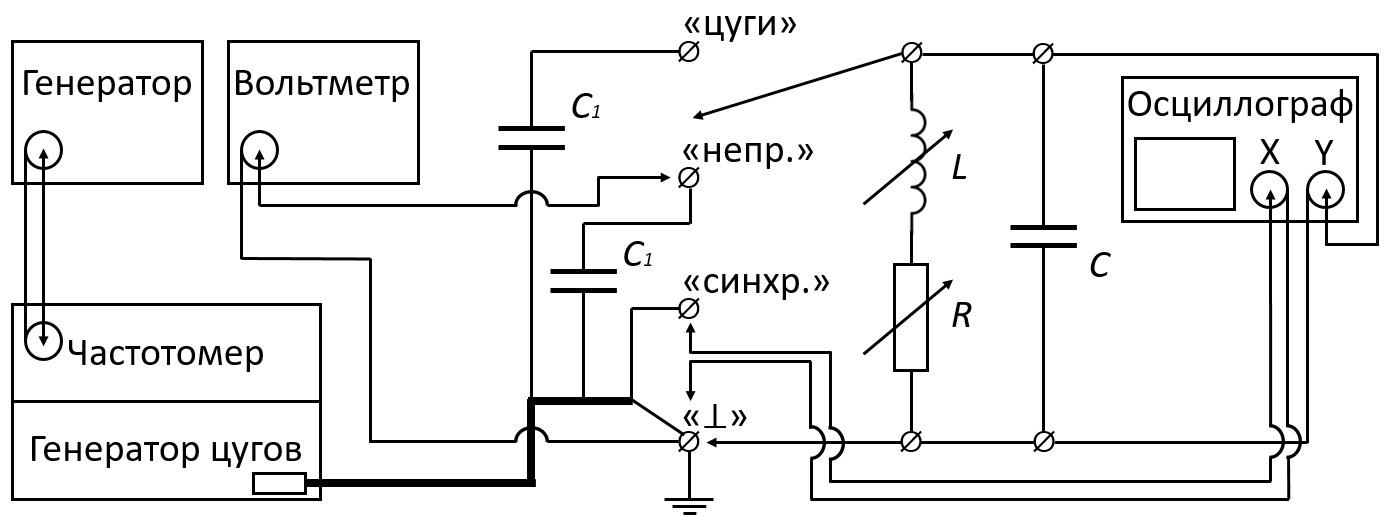
\includegraphics[width=6.49653in,height=2.48056in]{./media/image3.png}
\todo[author=Tiffani]{Рис. 19 немного не соответсвует рис. в ворд-файле}
Синусоидальное напряжение от звукового генератора проходит через
частотомер, позволяющий измерять рабочую частоту с высокой точностью, и
генератор цугов~---~электронное реле, ``разрезающее'' синусоиду на
периодически повторяющиеся цуги~---~отрезки синусоиды.

Затем сигнал через небольшую ёмкость $C_1$ поступает на клеммы,
смонтированные на отдельной панели. При подключении контура к клеммам
«$\perp$» и «непр.» на контур подаётся непрерывный сигнал~---~синусоида; если
контур подключён к клеммам «$\perp$» и «цуги»~---~на контур поступают отрезки
синусоиды.

Для наблюдения за процессом колебаний напряжение с ёмкости подаётся на
вход осциллографа. Чтобы картина на экране была устойчивой, частота
развёртки осциллографа принудительно синхронизуется с частотой
повторения цугов. Для этого на генератор развёртки ЭО подаются следующие
с частотой повторения цугов управляющие импульсы, которые вырабатываются
в блоке электронного реле (клемма «синхр», смонтированная на панельке).
Для измерений напряжения на ёмкости используется электронный вольтметр.

\begin{lab:task}

В работе предлагается при двух значениях сопротивления магазина
исследовать резонансные кривые и определить по ним добротность контура;
затем определить добротность, определив логарифмический декремент
затухания при нарастании и при затухании колебаний.

	\begin{enumerate}
	\tasksection{I. Подготовка приборов к работе}

	\item Соберите схему согласно рис.~\figref{forced oscillations exp scheme} и подключите контур к клеммам «$\perp$» и
«непр.». Включите приборы в сеть. Руководствуясь техническим описанием,
расположенным у установки, настройте генератор, осциллограф, проверьте
работоспособность источника питания, а также выставите необходимые
значения на магазинах сопротивлений и индуктивностей.

\tasksection{II.Исследование резонансных кривых}

	\item Рассчитайте собственную частоту контура
($\nu_{0} = 1/2\pi\sqrt{LC}$).

	\item Изменяя частоту генератора вблизи резонансной и наблюдая за
синусоидой на экране осциллографа, убедитесь, что в резонансе амплитуда
колебаний максимальна. Подберите частоту развёртки осциллографа и
амплитуду синхронизации, при которых картина неподвижна.

	\item Меняя частоту генератора в обе стороны от резонансной, снимите
зависимость показаний вольтметра $U$ от показаний частотомера
$\nu$. Расчёт добротности ведётся на уровне $0,7$ от резонансной
амплитуды, поэтому стоит аккуратнее провести измерения в районе этого
уровня, а также продолжать измерения по крайней мере до тех пор, пока
амплитуда сигнала упадёт до величины $0,3 - 0,4$ от резонансной.

	\item Установите на магазине сопротивлений другое значение, заданное
преподавателем, и повторите измерения п.4. Закончив измерения, отключите
вольтметр от сети.

\tasksection{III.Процессы установления и затухания колебаний}

	\item Подключите контур к клеммам «цуги» и «$\perp$». Выведите до нуля
сопротивление магазина.

	\item Установите на генераторе резонансную частоту. Подберите частоту
развёртки осциллографа, при которой на экране умещается один цуг
колебаний. Убедитесь, что огибающая затухающих колебаний это
перевёрнутая огибающая нарастающего участка. Если они заметно отличаются
(реле может внести искажения), то следует уменьшить амплитуду сигнала с
генератора.

	\item Для расчёта добротности по скорости нарастания амплитуды измерьте
амплитуды двух колебаний $U_k$ и $U_{k+n}$, разделённых целым числом периодов $n$,
и амплитуду установившихся колебаний $U_0$ (см. рис.~\figref{forced oscillations damping}).

Перед началом измерений заземлите канал $Y$, чтобы уточнить положение оси
$X$~---~начала отсчёта амплитуды. Можно увеличить амплитуду, сместив
горизонтальную ось симметрии цуга в нижнюю часть экрана. Расчёт будет
тем точнее, чем больше отличаются друг от друга все три амплитуды.

Проведите измерения для 3 -- 4-х пар амплитуд.

	\item Для определения добротности по скорости затухания измерьте две
амплитуды, разделённые целым числом периодов (для 3 -- 4-х пар амплитуд).

	\item Повторите измерения п.8 и п.9 для другого значения сопротивления,
заданного преподавателем.

	\item Сместите частоту генератора от резонансного значения и получите на
экране картину биений. Зарисуйте и объясните эту картину.

	\item Отключите приборы от сети и разберите схему.

	\item Измерьте активное сопротивление $R_L$ и индуктивность $L$ магазина
индуктивностей с помощью измерителя $LCR$ на частотах $50$~Гц, $500$~Гц и $1500$~Гц.

\tasksection{IV.Обработка результатов}

	\item Постройте на одном графике резонансные кривые в координатах $U/U0 = f(
\nu/\nu_0)$, где $U_0$~---~напряжение при резонансной частоте $\nu_0$.

Определите добротность по формуле $Q = \omega_0/(2\Delta\Omega)$. Сравните теоретическое и
экспериментальное значения резонансной частоты.

	\item Рассчитайте добротность контура по скорости нарастания и затухания
колебаний.

	\item Рассчитайте теоретическое значение добротности через параметры
контура $L$, $C$ и $R$.

	\item Сведите результаты определения $Q$ в таблицу:

	\begin{center}
\begin{tabular}{|c|c|c|c|c|c|}
\hline
& & \multicolumn{4}{c|}{$Q$}\\
\cline{3-6}
$R$, Ом & $R_{\text{конт}}$ & & & &$f(LCR)$\\
\hline
$0$ & & & & & \\
$100$ & & & & &\\
\hline
\end{tabular}
\end{center}
\todo[author=Tiffani]{Как вставить данные символы в таблицу(см. рисунок)?}

\begin{figure}[h!]
	\centering
	%\pic{0.6\linewidth}{Chapter_2/image4}
	\caption{Таблица}
\end{figure}

%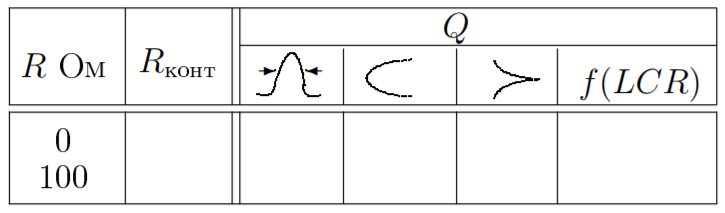
\includegraphics[width=3.37592in,height=0.99167in]{./media/image4.png}
	\item Оцените погрешности и сравните результаты расчётов.
	\end{enumerate}
\end{lab:task}

\todo[author=Tiffani]{Нет вопросов после лабораторной}

\begin{lab:literature}
	\item \emph{Сивухин~Д.В.} Общий курс физики. -- Т.III. Электричество. -- ~М.:~Физматлит,~2004. \S\S~122 -- 124.

	\item \emph{Калашников~С.Г.} Электричество. --~М.:~Физматлит, 2008. \S\S~207 -- 210.
\end{lab:literature}
